% $File: report.tex
% $Date: Sat Dec 14 17:08:44 2013 +0800
% $Author: wyx <ppwwyyxxc@gmail.com>

\documentclass[11pt,a4paper]{article}
\usepackage{threeparttable}
\usepackage{dirtree}
\usepackage{keystroke}


\usepackage{fontspec,amsmath,amssymb,zhspacing,verbatim,minted,listings,zhmath}
\usepackage{titlesec, titletoc}
\usepackage{pdfpages}
\usepackage{enumerate}
\usepackage[hyperfootnotes=false,colorlinks,linkcolor=blue,anchorcolor=blue,citecolor=blue]{hyperref}
\usepackage[backend=biber]{biblatex}
%\usepackage[dvips]{graphicx}
\usepackage{subfigure}
\usepackage{indentfirst}
\usepackage{float}			% don't automatically change location of figure [H]
\usepackage{chngpage}		% use \changetext to change page size
\usepackage{caption}\captionsetup{hypcap=true}  % ref to jump to object instead of caption
%\newfontfamily\zhfont[BoldFont=SimHei,ItalicFont=KaiTi_GB2312]{SimSun}
\lstset{keywordstyle=\color{blue!70}, commentstyle=\color{red!50!green!50!blue!50},frame=shadowbox,rulesepcolor=\color{red!20!green!20!blue!20},
basicstyle=\footnotesize\ttfamily}
\zhspacing
\setlength{\parindent}{2em}

\usepackage{fancyhdr}
\usepackage{array}

\changetext{}{2.2cm}{-1.1cm}{-1.1cm}{}
\pagestyle{fancy}
\setlength{\headheight}{15.2pt}
\lhead[]{}\rhead[]{}
\fancyhead[C]{\emph{Testing Document - Uknow InfoHub}}


%use cell in tabular
\newcommand{\tabincell}[2]{\begin{tabular}{@{}#1@{}}#2\end{tabular}}

%thick shline
\newlength\savewidth
\newcommand\shline{\noalign{\global\savewidth\arrayrulewidth\global\arrayrulewidth 1pt}
                   \hline
                   \noalign{\global\arrayrulewidth\savewidth}}


\defbibheading{bibliography}{\section{References}}
\bibliography{refs.bib}
\newcommand{\figref}[1]{\hyperref[fig:#1]{Fig. \ref*{fig:#1}}}
\newcommand{\secref}[1]{\hyperref[sec:#1]{Sec. \ref*{sec:#1}}}
\newcommand{\tabref}[1]{\hyperref[tab:#1]{Tab. \ref*{tab:#1}}}

% math function
\let\Oldsum\sum
\renewcommand{\sum}{\displaystyle\Oldsum}
\let\Oldprod\prod
\renewcommand{\prod}{\displaystyle\Oldprod}


../mint-defs.tex

\title{Uknow InfoHub \\ \small Design Document}
\author{BlXLRSMB Team}
\date{}

\begin{document}

\titleformat*{\section}{\centering\Large\bf}
\titleformat*{\subsubsection}{\large\bf}
\setlength{\baselineskip}{1.3em}
\fontsize{12}{\baselineskip}\selectfont



%
\includepdf{img/cover}
\maketitle
\tableofcontents
\clearpage

\newcolumntype{L}{>{\centering\arraybackslash}m{3cm}}

\section{Introduction}
\label{sec:intro}
\subsection{Document Introduction}
\label{sec:introduction}
	In the following sections of this document, we will present several skim of our project management.

	In~\secref{git}, how we use git as the subversion tool. Issues and milestones will be presented in~\secref{issue}.



\section{Test Scheme}
\label{sec:test_scheme}
  \subsection{Test Level}
    This test use method which simulating users' requests
    and determining whether whole project can response each request correctly.
    If project gives the correct response as design for one request, logic that get involved in generating response will be considered as tested.

    So, this test is on API level.

  \subsection{Test Environment}
    \subsubsection{Software Environment}
    \begin{table}[H]
        \begin{tabular}{c|c|c|c}
          \hline
          Name & Version & Purpose \\ \hline
          Python UnitTest & ~2.7 & Simulating Request for each API \\ \hline
          ApacheBench & >=2.3 & Performance Benchmark \\ \hline
        \end{tabular}
        \caption{Software Requirements\label{tab:Software}}
      \end{table}
    \subsubsection{Hardware Environment}
      In order to run the test, a POSIX machine is required.

\section{Test Procedure}
\label{sec:test_procedure}
\subsection{Testers}
zxytim, ppwwyyxx, vuryleo, jiakai
\subsection{Period}
18:00 Dec 13th, 2013 to 18:00 Dec 14th, 2013.
\subsection{Functional Tests}
\begin{enumerate}

  \item Test Case Designing
    First, read the API list, select out APIs that need to be tested.
    Then, design use cases for each API based on its function.
    At last, translate test cases into proper request format and add them into the test suite.

    Several cases that designed to test the robustness of the APIs are recorded as well.
    These cases will perform illegal requests such as requests with wrong format, permission overstep and injection.
  \item Environment Setting
    At first, use virtualenv to build a virtual python environment for this project.
    Then use install tool located in manage suite to set up runtime environment for it.

    In order to provide production environment, a mongodb server and a redis server is also required.
  \item Software Configuring
    In this test, the default configure is applied. So no interfere is needed in this step.
  \item Test Configuring
    In order to test some third party function, correct authentication information is required.
    The configure file can be found easily in test suite.
  \item Test Executing
    Execute test entry scripts to do the tests.
  \item Log Analyzing
    After getting the test log, parse out the useful information and ordinate them into proper format.

\end{enumerate}
\subsection{Performance Tests}
\subsubsection{Test Case Designing}
Several APIs that may have heavy loads are selected to get the performance data at the worse state.
Then a random set of APIs are generated in order to test the average performance.
Besides, APIs that are requested most frequently are selected to get the common performance.
\subsubsection{Environment Setting}
In propose of simulating real world performance,
client and server are located on different machines, so the network transform is considered.

To do so, deploy the project in production mode on one machine, and get the test suite on another.
\subsubsection{Test Executing}
Execute test entry scripts to do the tests.
\subsubsection{Log Analyzing}
Performance test will generate plenty of log.
So a data visualization procedure is taken to display the data in different collections and patterns.

\section{Test Result}
\label{sec:test_result}
  \subsection{Functional}
    All functional tests are passed. For more details please refer to~\appref{testcase}.
  \subsection{Performance}
	Here a sample of test result is presented. For detailed all plots, see appendix.
	\begin{figure}[!ht]
		\centering
		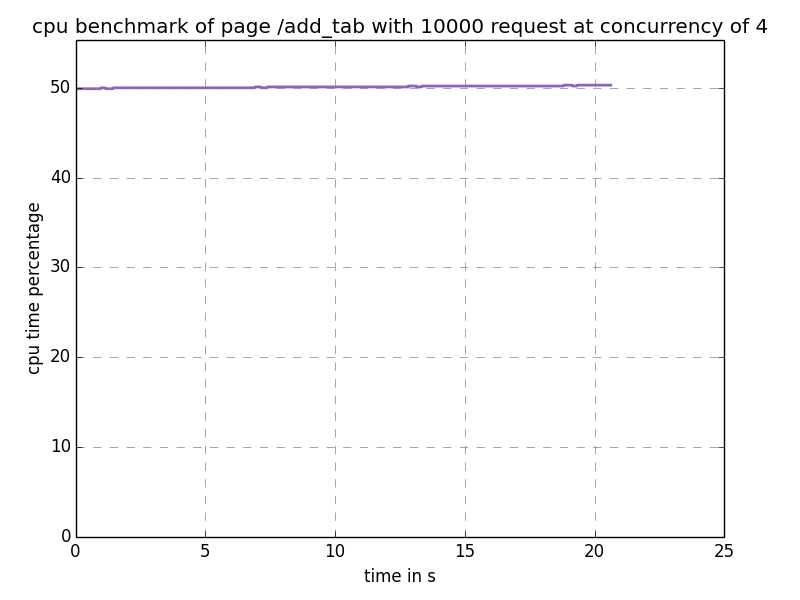
\includegraphics[width=0.5\linewidth]{img/add_tab.cpu.png}
		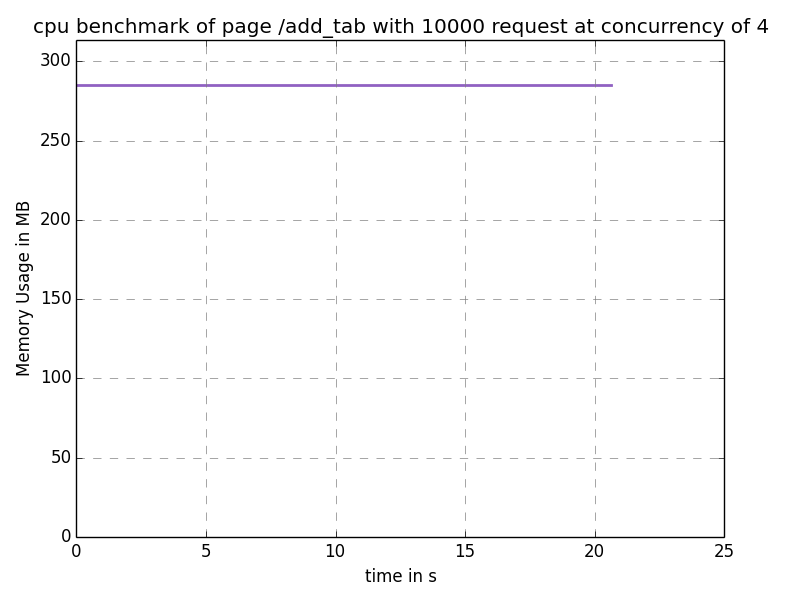
\includegraphics[width=0.5\linewidth]{img/add_tab.mem.png}
		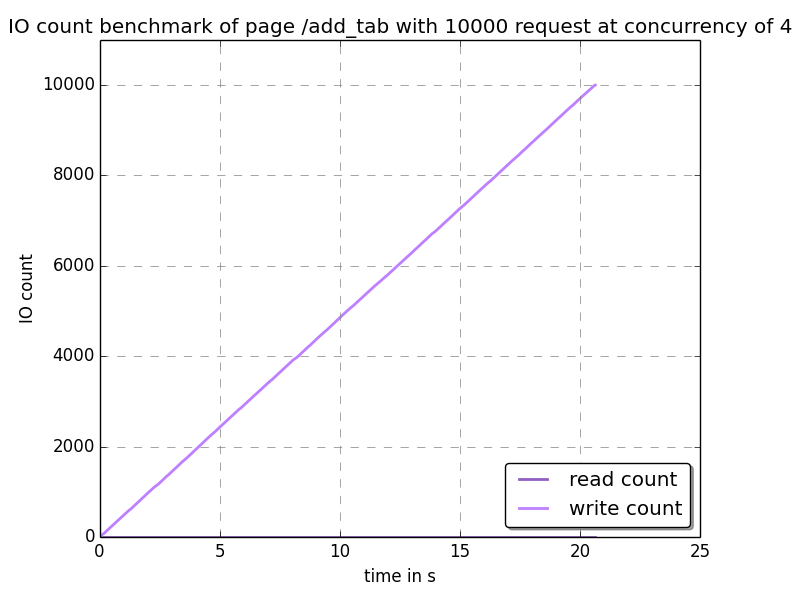
\includegraphics[width=0.5\linewidth]{img/add_tab.io-count.png}
		\caption{Test result of \textbf{add\_tab} API}
	\end{figure}
  \subsection{Converge}
    The converge ratio reached 90\%.
    For more details please refer to appendix converge sheet.

    The code that are not converged is mainly exception handle phase.
    But for each kind of exception handle, at least one case is designed to test it.
    For example, all most all APIs are login required,
    but only one test case that try to logout while not logged in is designed.
    For one kind of exception handle procedure is the same, but may occur in many situation.
    Designing duplicate test cases for each API doesn't means a lot but cause plenty of time.

    For others, they are designed for further widening usage that not implement yet.
    Such as more configurable fetcher, user defined color theme and so on.

\section{Test Evaluation}
\label{sec:test_evaluation}
  \subsection{Evaluation on the project}
    \subsubsection{Functional}
      All APIs work correctly as expected.
      And all APIs is robust even under sedulous injection or other kind of inroads.
      This result reveals the wise design of this project at the beginning and rich knowledge of the develop team in network security field.

    \subsubsection{Performance}
      Both average performance and common performance are quite well,
      but there are still work to do to speed up in the worst case.
      However, the enhancement is limited, since in the worst case, the API will return too much of data,
      and the bottleneck is therefore at network bandwidth.
      Therefore, an API for incremental request is needed in the future.
      This kind of API will remember what they have provided and won't return them again if not directly requested.

      Regardless of this, the worst response time is admissible by user, so further enhancement can be arrested until it really makes sense.

  \subsection{Evaluation on the test}
    \subsubsection{Functional}
      Functional test includes legal and illegal cases, considered boundary situation and uncommon use cases.
      Besides, many common injection cases are used, to test the security of the APIs.
      This part of test cases are completed and have covered many professional assault method.
    \subsubsection{Performance}
      For more detailed result to locate the bottleneck of the system, an enhancement for the performance test is needed.
      Current result only shows the response time for all APIs but doesn't have enough details, such as time spent on network transform and database
      query.

%
\includepdf{img/cover-normal}

\printbibliography

\end{document}

